\section{Planteamiento del problema}
\setcounter{sectiontotal}{4}

\begin{frame}
\frametitle{\pagetitle}
\framesubtitle{Descripción del problema}

%Aplicar los conceptos de los juegos serios en un área local para medir los
%factores que influyen en el diseño, la implementación y la evaluación de un
%juego serio.

%Este juego serio debe contemplar los siguientes factores.

\pause{}
\begin{itemize}[<+->]
    \item Implementación técnica.
    \item Adecuación para la educación.
    \item Integración total con los objetivos pedagógicos.
\end{itemize}

\end{frame}

\begin{frame}
\frametitle{\pagetitle}
\framesubtitle{Estado actual del Instituto Andrés Barbero}

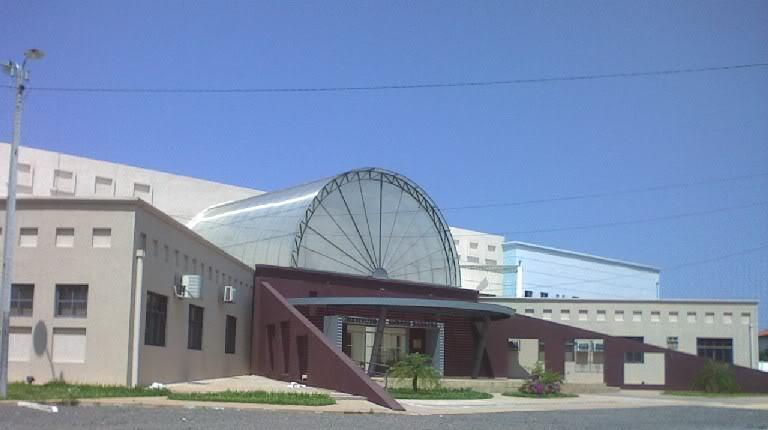
\includegraphics[width=\textwidth]{imagenes/iab.jpg} 

\end{frame}

\begin{frame}
\frametitle{\pagetitle}
\framesubtitle{Prácticas profesionales}

\begin{columns}
\column{.4\textwidth} \hspace{0.5cm}
\begin{overprint}
	 \onslide<1|handout:1> 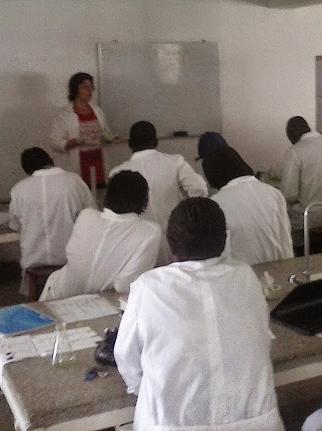
\includegraphics[width=\textwidth, height=5.5cm]{imagenes/clases_teoricas.png} 
    \onslide<2|handout:0> 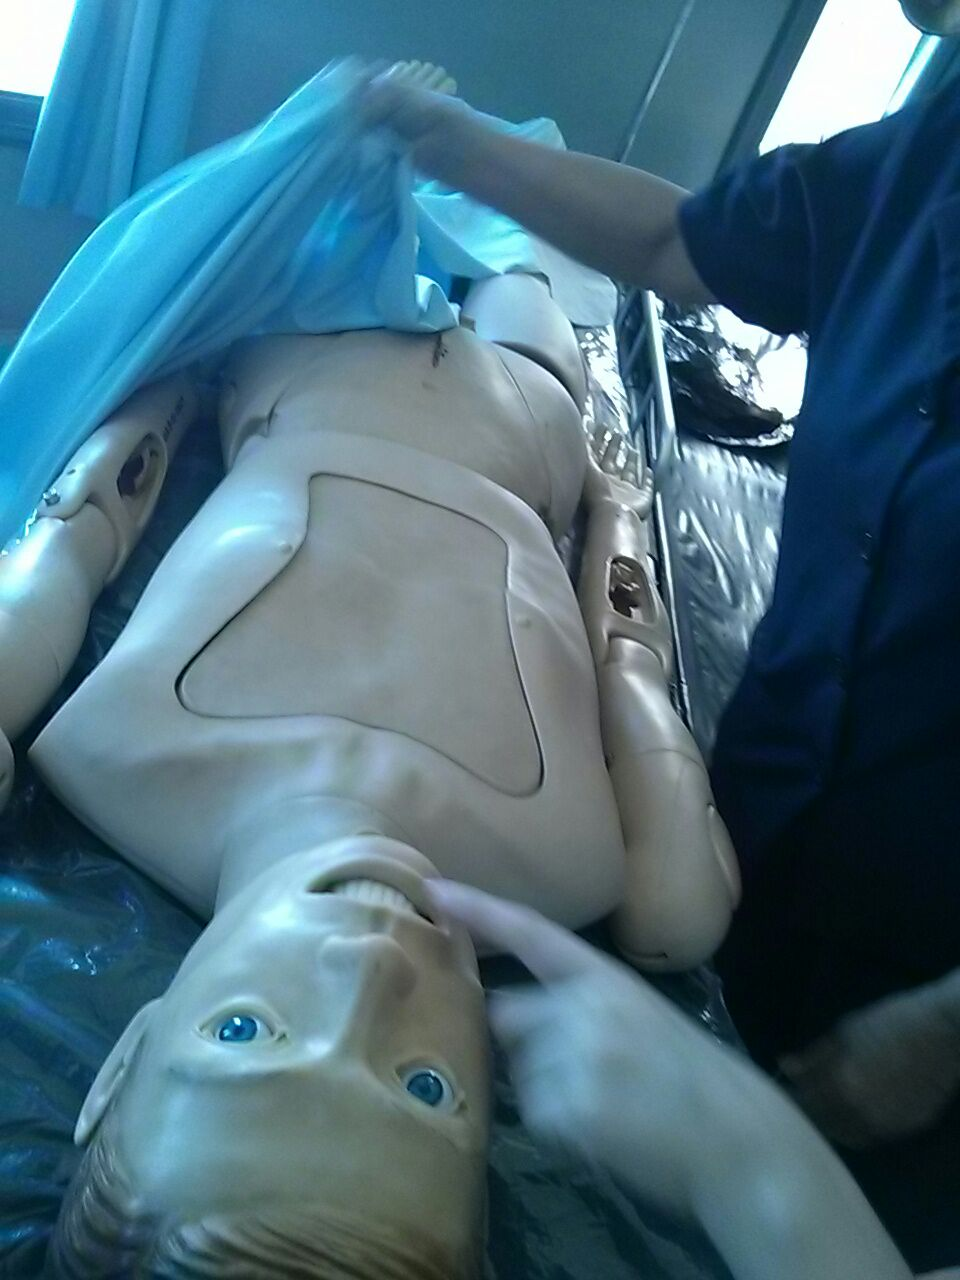
\includegraphics[width=\textwidth, height=5.5cm]{../problema/iab_sala_3.jpg} 
    \onslide<3|handout:0> 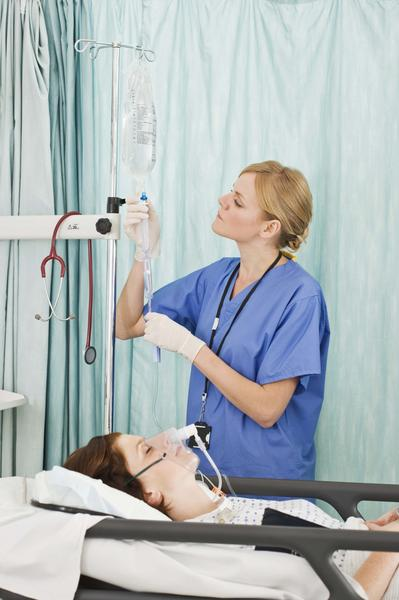
\includegraphics[width=\textwidth, height=5.5cm]{imagenes/practica_campo.jpg} 
   
\end{overprint}
\column{.7\textwidth} \hspace{0.5cm}
\begin{itemize}[<+->]
	\item Clases teóricas
	\item Prácticas en laboratorio
	\item Prácticas en hospitales o prácticas de campo
\end{itemize}
\end{columns}

\end{frame}

% Problemas actuales del Instituto Andrés Barbero
\begin{frame}
\frametitle{\pagetitle}
\framesubtitle{Problemas actuales del Instituto Andrés Barbero}
\begin{itemize}[<+->]
\item Preparación para las prácticas\sfcite{iab:tesis_alumnos}
\item Falta de tiempo\sfcite{iab:tesis_alumnos}.
\item Materiales desactualizados\sfcite{iab:tesis_alumnos}.
\item Cantidad de alumnos\footnote{Esta información se recabo en reuniones con
        los directores}

    \bigskip

    \begin{tabular}{lr}
        \tabitem{} Teoría   & 1:50 \\
        \tabitem{} Práctica & 1:10 \\
    \end{tabular}
\end{itemize}
\end{frame}

\section{Propuesta}
\setcounter{sectiontotal}{5}

% Descripción
\begin{frame}
\frametitle{\pagetitle}
\framesubtitle{Propuesta de solución}
\begin{block}{Descripción}
\centering
Desarrollo de un \textbf{Juego Serio} para dispositivos móviles que incluya la
simulación de laboratorios virtuales para apoyar el proceso de aprendizaje de
los alumnos de la carrera de enfermería, permitiendo a los mismos realizar
procedimientos de enfermería a un paciente virtual.
\end{block}
\end{frame}

% Criterios que resuelve
\begin{frame}
\frametitle{\pagetitle}
\framesubtitle{Motivación}

\begin{itemize}[<+->]
\item Evaluación
\item Progreso
\item Disponibilidad de tiempo
\item Factor psicológico
\item Enfoque individual
\end{itemize}
\end{frame}

\begin{frame}
\frametitle{\pagetitle}
\framesubtitle{Selección de contenido}

\begin{block}{Descripción}
\centering
Se seleccionaron dos procedimientos de enfermería: la \textbf{Venopunción} y 
la \textbf{Valoración de la escala de Glasgow}.
\end{block}

\end{frame}


% Venopunción
\begin{frame}
    \frametitle{\pagetitle}
    \framesubtitle{Venopunción}

    %\pause{}
    
    \begin{block}{Descripción}
    \centering
    El procedimiento denominado \emph{Venopunción} es utilizado
    frecuentemente para extraer muestras de sangre. Es un procedimiento invasivo
    que ofrece un medio directo de acceso al sistema vascular. 
    \end{block}

	\begin{columns}
	\column{.6\textwidth} \hspace{0.5cm}
    \centering
    \begin{tikzpicture}
      {\node[opacity=1]{%
              \includegraphicsx[width=.8\textwidth]{imagenes/extraccion.jpg}%
          };}
    \end{tikzpicture}
    
    \column{.5\textwidth} \hspace{0.5cm}
    \textbf{Competencia básica}
    \begin{itemize}
	\item Ayudar en procedimientos invasivos
	\end{itemize}
	\end{columns}

\end{frame}

\begin{frame}
    \frametitle{\pagetitle}
    \framesubtitle{Escala de Glasgow}
    
    \begin{block}{Descripción}
    \centering
    La escala de Glasgow es utilizada como una herramienta de valoración
    objetiva del estado de conciencia de pacientes en estado crítico. 
    
    Se evalúa la respuesta motora, verbal y ocular del paciente.
    \end{block}

	\begin{columns}
	\column{.6\textwidth} \hspace{0.5cm}
    \centering
    \begin{tikzpicture}
      {\node[opacity=.7]{%
              %\oldincludegraphics[width=.8\textwidth]{imagenes/glasgow.jpg}%
              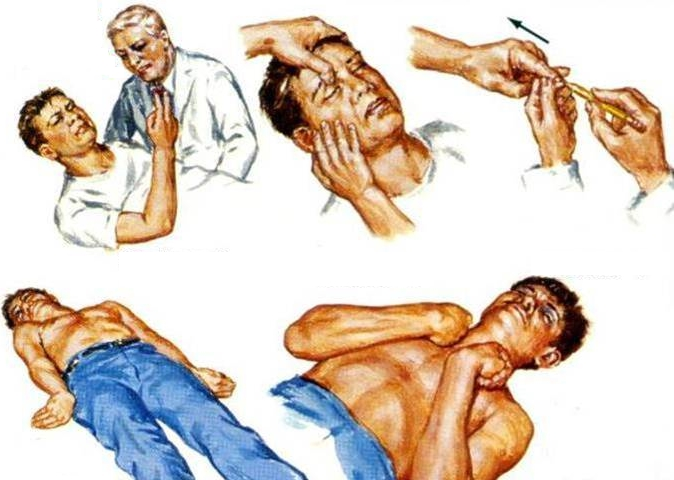
\includegraphics[width=.85\textwidth]{imagenes/glasgow.jpg}%
          };}
    \end{tikzpicture}
    
    \column{.5\textwidth} \hspace{0.5cm}
    \textbf{Competencia básica}
    \begin{itemize}
	\item Identificar actividades de cuidados según problemas urgentes principales.
	\end{itemize}
	\end{columns}

\end{frame}


